\documentclass[11pt]{article}
\usepackage[margin=1in]{geometry}
\usepackage[T1]{fontenc}
\usepackage{lmodern}
\usepackage{amsmath,amssymb,amsthm}
\usepackage{graphicx}
\usepackage{booktabs}
\usepackage{multirow}
\usepackage[numbers,sort&compress]{natbib}
\usepackage[colorlinks=true,linkcolor=blue,citecolor=blue,urlcolor=blue]{hyperref}
\usepackage{microtype}

\newcommand{\xv}{\mathbf{x}}
\newcommand{\uv}{\mathbf{u}}
\newcommand{\E}{\mathbb{E}}
\newcommand{\gttpp}{p_{\phi^\star}}
\newcommand{\selftpp}{p_{\psi}}

\title{Event-Timing Priors: Temporal Point Process Likelihoods Correct the
Long-Horizon Extreme-Event Statistics of Generative Surrogates}
\author{Gunner Howe\\ \texttt{gunnerlevihowe@gmail.com}}
\date{July 2026}

\begin{document}
\maketitle

\begin{abstract}
Generative surrogates of chaotic dynamical systems --- including modern
diffusion-based weather and climate emulators --- are routinely
\emph{evaluated} on extreme events but never \emph{trained} on their timing.
We show that this omission is consequential and correctable. Working with a
two-scale Lorenz-96 testbed observed under realistic conditions (coarse
emulator timestep, observation noise), we find that a conditional
flow-matching surrogate reproduces marginal statistics well while
systematically corrupting the \emph{temporal} statistics of
threshold-crossing extreme events in long rollouts: event rates inflate,
inter-event-time distributions distort, and return periods drift. We
introduce an \emph{event-timing prior}: a neural temporal point process (TPP)
fit to the event timings of a curated catalog, whose likelihood --- evaluated
on soft, differentiable events extracted from short surrogate rollouts ---
serves as an auxiliary fine-tuning signal. Naive likelihood maximization is
mode-seeking and collapses the event rate; we instead use a likelihood-ratio
objective against a co-trained ``self-TPP'' (the point-process analog of
variational score distillation), whose gradient vanishes exactly when the
surrogate's event process matches the catalog's. Across seeds, TPP-aux
fine-tuning recovers inter-event-time distributions, burstiness, and
return-period curves that invariant-measure matching \citep{jiang2023training}
provably leaves unconstrained, while a rate-matched Poisson control shows the
gains require the prior's temporal \emph{structure}, not merely its rate. A
second system (Kuramoto--Sivashinsky) maps the method's boundary: when
rollout \emph{dynamics} are deeply corrupted, a timing-only prior collapses
the event rate rather than repairing it --- a characteristic, easily
monitored failure signature whose mechanism we analyze. Event-timing
structure is thus a distinct, directly controllable axis of surrogate
quality --- one that complements, and does not substitute for,
dynamics-level training signals.
\end{abstract}

\section{Introduction}

Data-driven surrogates now emulate weather and climate at a fraction of the
cost of numerical models, and generative (diffusion-family) surrogates such
as GenCast \citep{price2025probabilistic} explicitly target probabilistic
skill. A striking asymmetry runs through this literature: extreme events ---
heat waves, cyclones, blocking episodes --- dominate the \emph{evaluation} of
these models \citep{price2025probabilistic,wattmeyer2025ace2,kochkov2024neural},
yet no training objective in use says anything about \emph{when} extremes
occur. Standard objectives constrain pointwise forecast error or, at best,
time-aggregated distributional statistics: invariant measures
\citep{jiang2023training,schiff2024dyslim}, spectra
\citep{chakraborty2026binned}, or adversarial OT statistics
\citep{melo2026learning}. All of these are invariant to permuting time ---
they cannot distinguish a process whose extremes arrive quasi-periodically
from one whose extremes arrive in bursts, so long as the marginals agree.

The temporal law of extremes is precisely what many downstream users care
about: return periods drive design codes; clustering of exceedances drives
compound risk; inter-event times drive recovery windows. And it is a
quantity for which independent, high-quality data often exists even when
state observations are noisy: curated event catalogs (hurricane best tracks,
earthquake catalogs, flood records) are compiled and quality-controlled
separately from gridded reanalyses.

This paper asks whether that timing information can be placed directly in
the training signal. We fit a small neural temporal point process (TPP) to
the event timings of a clean catalog and use its likelihood --- evaluated
on soft, differentiable events extracted from short surrogate rollouts,
via a likelihood-ratio construction that we show is necessary to avoid
mode collapse --- as an auxiliary fine-tuning objective for a conditional
flow-matching surrogate. On a two-scale Lorenz-96 testbed observed at a
coarse timestep under observation noise, eight-seed paired experiments
show the resulting surrogate's long-rollout event process becomes
statistically indistinguishable from truth under the catalog TPP, with
event rates, inter-event-time distributions, and return-period curves
restored at a ${\sim}0.5\%$ cost in short-horizon skill --- while matched
controls (rate-only priors, invariant-measure objectives, rollout
stabilizers) each leave a characteristic part of the deficit in place. A
second system (Kuramoto--Sivashinsky) delimits where the approach applies:
when the rollout \emph{dynamics} themselves are deeply corrupted, a
timing-only prior collapses the event rate instead of repairing it, by a
mechanism we analyze.

\textbf{Contributions.}
\begin{enumerate}
  \item We demonstrate a clean dissociation: under realistic training
  conditions (coarse timestep, noisy observations), a strong generative
  surrogate's long-horizon rollouts corrupt event-timing statistics, and
  the most consequential components of that corruption --- return periods,
  burstiness, the conditional intensity of events --- are exactly the ones
  invariant-measure/marginal-statistics training leaves unrepaired
  (\S\ref{sec:results}).
  \item We introduce TPP-aux fine-tuning: a neural TPP fit to catalog event
  timings acts as a differentiable prior on the timing of soft events
  extracted from short surrogate rollouts (\S\ref{sec:method}). We identify
  and solve the mode-seeking pathology of naive TPP-likelihood maximization
  via a likelihood-ratio (self-TPP) objective, the point-process analog of
  variational score distillation \citep{wang2023prolificdreamer,luo2023diffinstruct}.
  \item Controls that isolate the mechanism: a rate-matched
  \emph{Poissonized} TPP prior (same loss form and strength, no temporal
  structure) actively damages event timing rather than repairing it; the
  invariant-measure objective of \citet{jiang2023training} (given equally
  privileged clean statistics) excels at marginals but leaves return
  periods and burstiness unrepaired; pushforward-style stabilization
  \citep{brandstetter2022message} improves rate-side statistics without
  learning conditional timing structure, at a significant cost to spectra
  and probabilistic skill.
  \item An honest map of the method's boundary: on Kuramoto--Sivashinsky,
  where the base surrogate's rollout \emph{dynamics} are deeply corrupted
  (spectrum errors of $e^{3}$) despite near-perfect state marginals, every
  timing-only variant collapses the event rate --- we analyze the
  mechanism (mode-seeking through the only accessible descent direction,
  outrunning the self-TPP brake) --- and neither dynamics-level objectives
  nor naive composition fully recovers the event process
  (\S\ref{sec:ks}).
\end{enumerate}

\section{Related work}
\label{sec:related}

\textbf{Long-time statistics of neural surrogates.}
\citet{jiang2023training} train neural operators to preserve invariant
measures of chaotic attractors via an optimal-transport (Sinkhorn) loss on
physics-informed summary statistics, or a contrastive feature loss; DySLIM
\citep{schiff2024dyslim} regularizes toward the invariant measure; spectral
losses match frequency content \citep{chakraborty2026binned}; adversarial OT
regularization matches trajectory statistics \citep{melo2026learning}.
These objectives are functions of the \emph{time-marginal} (or
time-averaged) law of the process and are therefore blind to the ordering
and spacing of rare events; we use \citet{jiang2023training} as our primary
control. Rollout stabilization --- the pushforward trick
\citep{brandstetter2022message}, noise injection and refinement
\citep{pedersen2025thermalizer,liu2026selfrefining}, Jacobian regularization
\citep{nie2026jaws} --- targets stability, an orthogonal axis.

\textbf{Extremes and generative emulators.}
\citet{stamatelopoulos2025diffusion} study when diffusion models extrapolate
amplitude tails; \citet{manshausen2026accurate} extract extreme-event
likelihoods from a trained diffusion emulator at inference time. Flagship
emulators evaluate extremes diagnostically
\citep{price2025probabilistic,wattmeyer2025ace2,kochkov2024neural}. None of
these place event \emph{timing} in the training signal.
The extreme-event-aware learning line of the Sapsis school brings extremes
into the \emph{training} signal --- via output-weighted risk functionals
and active sampling of dangerous states \citep{pickering2022discovering},
or by enforcing the amplitude statistics of an extremeness observable as a
statistical regularizer ($\eta$-learning, \citealp{chang2025extreme}) ---
but in both cases the constraint concerns \emph{which states} matter or
how extreme \emph{amplitudes} are distributed, not \emph{when} events
occur: the temporal law of the event process in long generative rollouts
remains unconstrained, which is precisely the axis we target.
\citet{raeth2026decision} augment generative forecasters with differentiable
decision losses --- structurally the closest training-objective precedent ---
but target decision cost, not temporal event structure, and no dynamical
rollout is involved.

\textbf{Neural temporal point processes.}
Neural TPPs model conditional intensities of event sequences
\citep{mei2017neural} or inter-event densities directly
\citep{shchur2020intensity}; see \citep{aalaila2026seahorse} for
benchmarking. To our knowledge, TPP likelihoods have not previously been
used as training objectives for dynamical-system surrogates.

\section{Method}
\label{sec:method}

\subsection{Setup: surrogates, events, catalogs}

Let $\xv_t \in \mathbb{R}^K$ be the observed (slow) state of a chaotic system
sampled at interval $\Delta t$. A generative surrogate models
$p_\theta(\xv_{t+1} \mid \xv_t)$; long rollouts compose samples
autoregressively. We train on noisy observations
$\tilde\xv_t = \xv_t + \varepsilon_t$,
$\varepsilon_t \sim \mathcal{N}(0, r^2\sigma_x^2 I)$, reflecting the
practical setting where state data comes from noisy analyses
\citep{jiang2023training}.

Events are threshold upcrossings of a scalar site observable $s_k(t)$
(here $s_k = -x_k$, deep troughs; threshold $u$ = the pooled 95th
percentile): an event occurs at step $t$ of stream $k$ iff $s_k(t) > u$ and
$s_k(t-1) \le u$. By rotational symmetry the $K$ site streams are
exchangeable. We assume access to a \emph{catalog}: the event timings
extracted from the clean historical record (in practice, curated event
databases; in our testbed, events of the clean trajectories underlying the
noisy training data). Crucially, the catalog contains \emph{event times
only} --- orders of magnitude less information than the full state record.

\subsection{The event-timing prior: a recurrent-intensity TPP}

We fit a discrete-time recurrent-intensity TPP $\gttpp$ to catalog streams:
a GRU consumes the binary event sequence $w_{1:T}$ of one stream and emits a
per-step conditional intensity $\lambda_t = \mathrm{softplus}(g(h_{t-1}))$
(events per unit time, depending only on events strictly before $t$), with
log-likelihood
\begin{equation}
\label{eq:tpp-ll}
\mathcal{L}(w; \lambda) \;=\; \sum_t \big[\, w_t \log \lambda_t
 \;-\; \lambda_t\, \Delta t \,\big],
\end{equation}
the standard grid discretization of the continuous point-process likelihood
\citep{daley2003introduction,mei2017neural}, exact as $\Delta t \to 0$.
Two properties matter. First, \eqref{eq:tpp-ll} is \emph{linear in} $w_t$,
so relaxed (soft) event indicators substitute cleanly --- this is what makes
the prior differentiable end-to-end. Second, the same fitted model
evaluates any candidate event stream, which is how it becomes a training
signal.

\subsection{Soft events from differentiable rollouts}

From a rollout $\hat\xv_{0:T}$ we extract soft upcrossing weights
\begin{equation}
w_t \;=\; \sigma\!\big((s_t - u)/\tau\big)\,
          \sigma\!\big((u - s_{t-1})/\tau\big) \in [0,1],
\end{equation}
with temperature $\tau$ calibrated so the soft event rate matches the hard
rate on held-out data (bias $<5\%$ at our $\tau$). The surrogate's few-step
deterministic sampler makes each rollout step differentiable given its
noise draw, and gradients through the chaotic dynamics are truncated to
windows of $T_w$ steps (states are recorded in a gradient-free rollout, and
all windows are re-forwarded with gradients in parallel from their recorded
start states --- identical values and gradient semantics to truncated BPTT,
at a fraction of the sequential cost). The TPP consumes the full stream:
each rollout is prefixed with the catalog's event history preceding the
initial condition, so intensities are history-calibrated where the
likelihood begins to count.

\subsection{Mode-seeking, and the likelihood-ratio fix}
\label{sec:ratio}

The obvious auxiliary loss, $-\E[\mathcal{L}(w^{\mathrm{soft}};
\lambda_{\phi^\star})]$, is a density, not a fit measure: under a fitted
TPP the \emph{empty} sequence often has higher density than typical
sequences, so maximizing catalog-TPP likelihood of rollout events drives
the surrogate toward the TPP's mode --- suppressing events rather than
matching their law. We observe exactly this collapse empirically
(\S\ref{sec:ablations}).
The fix mirrors variational score distillation
\citep{wang2023prolificdreamer,luo2023diffinstruct}: maintain a small
\emph{self-TPP} $\selftpp$, refit continually by maximum likelihood on the
surrogate's own (hard, detached) rollout events, and optimize the ratio
\begin{equation}
\label{eq:ratio}
\mathcal{L}_{\mathrm{aux}}(\theta) \;=\;
 -\,\E_{\mathrm{rollouts}}\big[\,
 \mathcal{L}(w^{\mathrm{soft}}; \lambda_{\phi^\star})
 - \mathcal{L}(w^{\mathrm{soft}}; \lambda_{\psi})\,\big].
\end{equation}
In expectation this is the reverse KL between the surrogate's event process
and the catalog process (up to the self-TPP's fit error): its gradient
vanishes exactly when the two laws agree, and the self-TPP term cancels the
uniform ``fewer events are more likely'' pressure. Fine-tuning minimizes
$\mathcal{L}_{\mathrm{FM}} + \lambda_{\mathrm{aux}} \mathcal{L}_{\mathrm{aux}}$,
keeping the base flow-matching loss as an anchor on ordinary skill.

\subsection{Conditions}
\label{sec:conditions}

All conditions fine-tune the \emph{same} per-seed base checkpoint for the
same number of steps; they differ only in the auxiliary objective:
\textbf{base} (flow-matching only, compute-matched);
\textbf{TPP-aux} (ours, Eq.~\ref{eq:ratio} with the catalog TPP);
\textbf{Poisson-aux} (identical, but the prior TPP is fit to Poissonized
catalogs --- same rate, exponential inter-event times; the
content-specificity control);
\textbf{invariant-stats} (the OT objective of \citet{jiang2023training}:
debiased Sinkhorn divergence between rollout and clean-climatology clouds of
their physics-informed summary statistics $\{\dot u_i,
(u_{i+1}-u_{i-2})u_{i-1}, u_i\}$ --- given the same clean-reference
privilege as the catalog);
\textbf{pushforward} \citep{brandstetter2022message};
\textbf{deterministic} (MSE-trained autoregressive baseline).

\section{Experimental setup}
\label{sec:setup}

\textbf{System.} Two-scale Lorenz-96 \citep{lorenz1996predictability,
wilks2005effects}: $K{=}40$ slow sites, $J{=}10$ fast variables per site
($F{=}10$, $h{=}1$, $b{=}c{=}10$), RK4 at $dt{=}0.002$, observed at
$\Delta t = 0.2$ MTU (coarse emulator step). Training: 64 trajectories
$\times$ 160 MTU with observation noise $r{=}0.3$; evaluation references
from clean held-out runs (26{,}600 MTU total).

\textbf{Ground-truth event structure.} Trough events are strongly
sub-Poisson (quasi-periodic recurrence): IET CV $0.78$, Fano factors
$0.6$--$0.7$ across windows; near-renewal (lag-1 IET correlation
$\approx 0$). Aggregate (spatial-max) events are super-Poisson (CV $1.15$)
--- used as a held-out transfer diagnostic.

\textbf{Models.} Surrogate: conditional flow matching
\citep{lipman2023flow} on normalized state residuals; 1D circular CNN
(4 residual blocks, width 96, FiLM noise-level conditioning, $\sim$0.66M
parameters); 6-step Euler sampler. TPP: single-layer GRU, hidden 64
($\sim$40k parameters). Full hyperparameters in appendix.

\textbf{Metrics.} Event timing: pooled IET distribution (two-sample KS,
$W_1$), event rate ratio, Fano-factor curve error, return-period curves at
catalog quantiles $q \in \{0.9,\dots,0.995\}$, catalog-TPP held-out
log-likelihood of rollout events. Ordinary skill: pooled state $W_1$, PSD
log-distance, ACF error, short-horizon CRPS and ensemble spread. Stability:
diverged-rollout fraction (censored and reported). Eight confirmatory
seeds, paired by shared base checkpoint; the tuning seed is excluded.

\section{Results}
\label{sec:results}

\subsection{Lorenz-96: the event-timing deficit and its repair}

All numbers: mean $\pm$ s.d.\ over eight confirmatory seeds, paired by
shared base checkpoint; $p$-values are paired $t$-tests against the base
condition (two-sided Wilcoxon agrees; it reaches its $n{=}8$ floor of
$0.008$ on every headline metric below unless noted).

\textbf{The base surrogate corrupts event timing.} Trained on noisy
observations, the base surrogate's long rollouts ($64 \times 800$ MTU)
inflate the event rate by $10.7\% \pm 1.4\%$, distort the inter-event-time
distribution (IET KS $0.068 \pm 0.007$, $W_1$ $0.44 \pm 0.05$ MTU), and
shift return periods (mean $|\log \mathrm{RP}_{\mathrm{model}} /
\mathrm{RP}_{\mathrm{true}}|$ $= 0.113 \pm 0.014$ across catalog quantiles
$0.90$--$0.995$). An identically-budgeted continuation of flow-matching
training (\textbf{base} condition) leaves all of these unchanged --- the
deficit is persistent, not undertraining.

\textbf{TPP-aux repairs it without costing skill.} Fine-tuning with the
event-timing prior recovers the event rate ($1.001 \pm 0.029$;
$p=8\!\times\!10^{-5}$), the IET distribution (KS $0.026 \pm 0.009$,
$p=3\!\times\!10^{-5}$; $W_1$ $0.13 \pm 0.06$, $p=1\!\times\!10^{-5}$),
and return periods ($0.052 \pm 0.028$, $p=0.002$). The catalog-TPP
log-likelihood of rollout events rises to $-0.0988 \pm 0.0013$ ---
statistically indistinguishable from the value the catalog TPP assigns to
\emph{real} held-out event sequences ($-0.0994$): the fine-tuned
surrogate's events are exactly as typical under the prior as truth itself,
neither less (deficit) nor more (mode-seeking). Short-horizon CRPS changes
by $+0.5\%$ ($p=0.048$; Wilcoxon $p=0.078$) --- a marginal cost two
orders of magnitude ($\sim$170$\times$) smaller than the deterministic
baseline's gap; no rollout diverged in any condition
(Table~\ref{tab:main}).

\textbf{Structure, not rate: the Poisson control.} The Poissonized prior
--- identical loss form, identical strength, identical rate information,
exponential inter-event times --- does not merely fail; it actively damages
the surrogate (IET $W_1$ $0.98 \pm 0.22$, $p=4\!\times\!10^{-4}$; rate
ratio $0.82 \pm 0.03$, $p=3\!\times\!10^{-8}$; Fano error $+0.056$,
$p=1\!\times\!10^{-5}$). Its rollouts' hazard function is driven toward a
constant (Fig.~\ref{fig:hazard}), erasing the quasi-periodic recurrence
structure the dynamics should carry: optimizing toward a structureless
event law distorts the dynamics that produce events. The gains of TPP-aux
are therefore attributable to the \emph{temporal structure} of the prior,
not to rate matching or to the loss mechanics.

\textbf{What the timing prior transfers.} Ground-truth trough events are
quasi-periodic: the IET distribution is multimodal at harmonics of the
wave-recurrence period, and the conditional hazard oscillates
(Fig.~\ref{fig:hazard}, black). The base surrogate over-amplifies the
hazard oscillation; TPP-aux pulls it onto the ground-truth curve; the
Poisson prior flattens it. On the IET quantile--quantile plot
(Fig.~\ref{fig:iet}), TPP-aux is the only condition tracking the diagonal
across the full range.

\textbf{Comparison with time-marginal objectives.} The invariant-statistics
control \citep{jiang2023training}, given clean summary-statistic clouds of
equal privilege, achieves the best state marginals and spectra (as
designed) and --- in this noise-dominated regime, where the base's timing
errors are largely inherited from amplitude corruption --- also improves
IET-level statistics. But it does not improve return periods
($0.107 \pm 0.036$ vs.\ base $0.113$, $p=0.73$), marginally worsens
burstiness (Fano error $0.045$ vs.\ $0.033$, $p=0.057$), undershoots the
event rate ($0.970$), and its rollout events are \emph{more} typical than
truth under the catalog TPP ($-0.0976$, overshooting the ceiling). The
pushforward control improves rate-side statistics (return periods
$0.039 \pm 0.009$) --- consistent with its denoising effect on rollouts
--- but leaves the conditional timing structure untouched (catalog-TPP LL
$-0.1012$, at base level) and significantly degrades spectra
($p=10^{-8}$) and CRPS ($p=3\!\times\!10^{-8}$). Only TPP-aux exhibits the full pattern:
conditional timing at the ground-truth ceiling, marginals improved, and
ordinary skill preserved. The deterministic AR baseline, for reference, is
far worse on every axis (CRPS $3.23$ vs.\ $1.74$; state $W_1$ $0.47$),
confirming that generative surrogates are the right object of study.

\begin{table}[t]
\centering
\caption{Lorenz-96 main results: mean $\pm$ s.d.\ over confirmatory seeds
(shared base checkpoint per seed; identical fine-tuning budgets). Bold =
best among fine-tuned generative conditions. IET = inter-event time;
RP = return period; TPP-LL = catalog-TPP log-likelihood of rollout events
(ground-truth ceiling $-0.0994$); CRPS at lead 20 steps.}
\label{tab:main}
\resizebox{\textwidth}{!}{\begin{tabular}{lccccccc}
\toprule
condition & IET KS & IET $W_1$ & rate ratio & RP log-err & TPP-LL & state $W_1$ & CRPS@20 \\
\midrule
Base (FM only) & $0.068 \pm 0.007$ & $0.438 \pm 0.050$ & $1.106 \pm 0.014$ & $0.113 \pm 0.014$ & $-0.1020 \pm 0.0003$ & $0.100 \pm 0.013$ & $\mathbf{1.735 \pm 0.002}$ \\
\textbf{TPP-aux (ours)} & $0.026 \pm 0.008$ & $\mathbf{0.128 \pm 0.056}$ & $\mathbf{1.001 \pm 0.029}$ & $0.052 \pm 0.027$ & $-0.0988 \pm 0.0013$ & $0.067 \pm 0.047$ & $1.744 \pm 0.009$ \\
Poisson-TPP-aux & $0.088 \pm 0.018$ & $0.977 \pm 0.222$ & $0.821 \pm 0.034$ & $0.203 \pm 0.087$ & $\mathbf{-0.0952 \pm 0.0017}$ & $0.156 \pm 0.029$ & $1.769 \pm 0.013$ \\
Invariant-stats & $\mathbf{0.025 \pm 0.008}$ & $0.181 \pm 0.088$ & $0.970 \pm 0.028$ & $0.107 \pm 0.035$ & $-0.0976 \pm 0.0013$ & $\mathbf{0.041 \pm 0.018}$ & $1.751 \pm 0.016$ \\
Pushforward & $0.047 \pm 0.002$ & $0.147 \pm 0.020$ & $1.031 \pm 0.006$ & $\mathbf{0.038 \pm 0.009}$ & $-0.1012 \pm 0.0002$ & $0.080 \pm 0.008$ & $1.768 \pm 0.003$ \\
Deterministic AR & $0.158 \pm 0.066$ & $0.945 \pm 0.361$ & $1.276 \pm 0.157$ & $0.396 \pm 0.207$ & $-0.1013 \pm 0.0092$ & $0.466 \pm 0.120$ & $3.227 \pm 0.020$ \\
\bottomrule
\end{tabular}}
\end{table}

\begin{figure}[t]
\centering
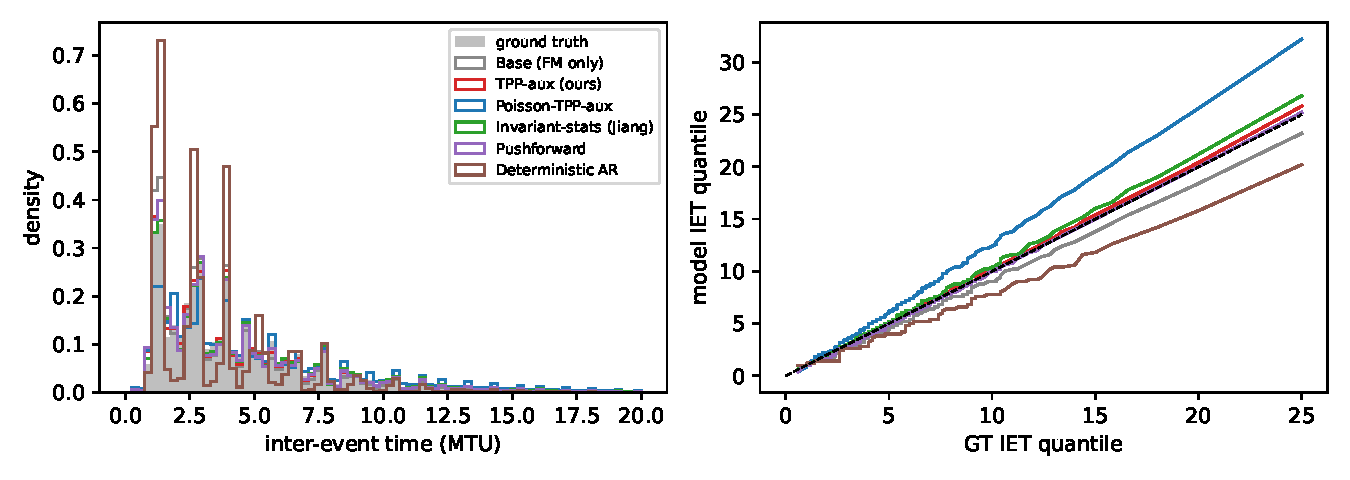
\includegraphics[width=\textwidth]{figs/iet.pdf}
\caption{Inter-event-time statistics, Lorenz-96 (pooled over 8 seeds).
Left: IET densities; ground truth (shaded) is multimodal at wave-recurrence
harmonics. Right: quantile--quantile against ground truth; TPP-aux (red)
tracks the diagonal; the Poissonized prior (blue) severely distorts the
distribution.}
\label{fig:iet}
\end{figure}

\begin{figure}[t]
\centering
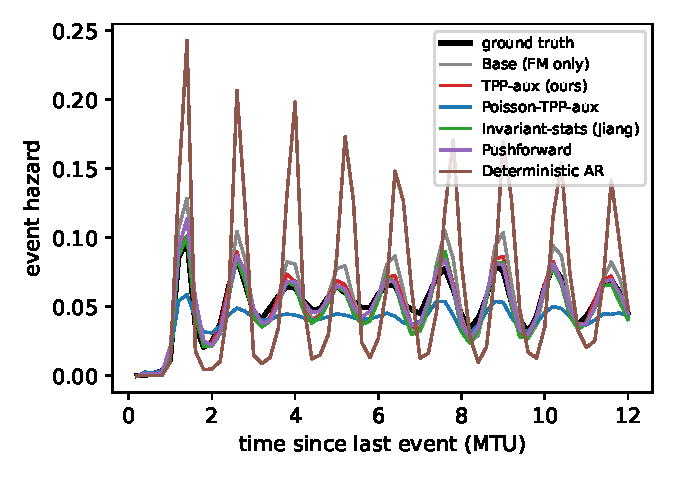
\includegraphics[width=0.55\textwidth]{figs/hazard.pdf}
\caption{Conditional event hazard vs.\ time since the last event. Ground
truth (black) oscillates at the recurrence period. The base surrogate
over-amplifies the oscillation; TPP-aux (red) matches it; the rate-matched
Poisson prior (blue) flattens it --- the content-specificity dissociation
in a single curve.}
\label{fig:hazard}
\end{figure}

\subsection{Kuramoto--Sivashinsky: the boundary of a timing-only prior}
\label{sec:ks}

KS ($L=22$, $N=64$, $\Delta t = 1$ tu; events = upcrossings of $u$ at its
95th percentile, \emph{clustered}, IET CV $1.58$ --- the opposite deviation
from Poisson to Lorenz-96) probes a qualitatively different deficit. The
noisy-observation base surrogate's rollouts have a nearly perfect state
marginal (state $W_1 = 0.037$) but a severely corrupted event process
($2.5\times$ the true rate; IET KS $0.59$; return-period log-error $1.14$)
driven by a \emph{deep dynamical} corruption: the rollout power spectrum is
wrong by $e^{3}$ at high frequencies --- jittery dynamics generating
spurious threshold re-crossings. This is the setting the introduction's
logic points to: nothing here is fixable by matching state marginals alone.

The outcome inverts Lorenz-96, and is instructive. \textbf{The timing-only
prior fails, by a characteristic mechanism.} Under TPP-aux the event rate
collapses to $0.31$ of truth (IET $W_1$ worsens from $55$ to $180$), and
the collapse persists across auxiliary weights $\{1,3,10\}$, self-TPP
budgets $\{5,25\}$ steps, gentler and $3\times$ longer fine-tuning, and a
milder noise level ($r{=}0.2$; rate $0.19$). The training traces show why:
a clustered prior assigns very low baseline intensity between bursts, so
each of the base model's many mistimed events is heavily penalized, and
within ${\sim}200$ steps the surrogate's event process shoots \emph{past}
the target into sparsity while the self-TPP lags; once the self-TPP
catches up, the two likelihoods equilibrate ($\mathcal{L}_{\phi^\star}
\approx \mathcal{L}_{\psi}$, both above the ground-truth ceiling) and the
residual KL pressure ($\approx 0.005$/step) is too weak against the
flow-matching anchor to escape. In short: when the underlying dynamics are
too corrupted to offer a gradient direction that \emph{places} events
correctly, suppressing events is the accessible descent path, and the
ratio objective's correct fixed point is unreachable. Suppression---not
repair---is the failure signature to monitor (the rollout event rate makes
it visible immediately).

\textbf{The controls invert accordingly} (Table~\ref{tab:ks}). The
rate-matched \emph{Poisson} prior --- harmful on Lorenz-96 --- is the best
return-period condition on KS (RP log-error $0.16$; rate $0.96$): where
the dominant error \emph{is} the rate, a rate-only prior transfers exactly
the information that is broken, and its permissive constant hazard exerts
no placement pressure that the corrupted dynamics cannot satisfy. The two
systems are mirror images: a prior helps precisely to the extent that its
content matches the deficit, and a structured prior whose structure the
dynamics cannot realize does damage instead.

\textbf{What does repair KS's temporal structure is a dynamics-level
statistic.} The \citet{jiang2023training} objective --- whose KS summary
statistics include the \emph{temporal increment} $u_t$, a local-dynamics
constraint rather than a pure time-marginal --- repairs the spectrum
($3.40 \to 1.83$) and with it most of the event statistics (rate $1.03$,
IET KS $0.26$), though substantial timing error remains (IET $W_1$ $22$
vs.\ a base of $55$; Fano error $0.34$): no condition fully recovers the
KS event process. Composing the two priors (climatology + catalog)
reaches the correct typicality level (catalog-TPP LL at the ceiling) and
more than halves the base IET KS ($0.22 \pm 0.05$), but the timing term
still drags the rate down ($0.72 \pm 0.08$) relative to the increment
objective alone --- the priors do not simply add.

\begin{table}[t]
\centering
\caption{Kuramoto--Sivashinsky results (3 seeds). Ground-truth
catalog-TPP ceiling: $-0.050$. The
timing-only prior collapses the event rate; the rate-only (Poisson) prior
--- harmful on Lorenz-96 --- is here the best return-period condition;
increment statistics ($u_t$) repair the dynamics and most of the timing.}
\label{tab:ks}
\resizebox{\textwidth}{!}{\begin{tabular}{lccccccc}
\toprule
condition & IET KS & IET $W_1$ & rate ratio & RP log-err & TPP-LL & state $W_1$ & PSD log-dist \\
\midrule
Base (FM only) & $0.594 \pm 0.002$ & $54.6 \pm 0.0$ & $2.50 \pm 0.00$ & $1.14 \pm 0.00$ & $-0.162 \pm 0.000$ & $0.037 \pm 0.001$ & $3.40 \pm 0.00$ \\
TPP-aux & $0.464 \pm 0.128$ & $179.5 \pm 11.6$ & $0.31 \pm 0.01$ & $1.92 \pm 0.18$ & $-0.025 \pm 0.001$ & $0.234 \pm 0.027$ & $3.15 \pm 0.01$ \\
Poisson-TPP-aux & $0.232 \pm 0.011$ & $35.7 \pm 1.0$ & $0.96 \pm 0.03$ & $0.16 \pm 0.01$ & $-0.065 \pm 0.002$ & $0.156 \pm 0.034$ & $3.04 \pm 0.05$ \\
Invariant-stats (incl.\ $u_t$) & $0.262 \pm 0.025$ & $22.3 \pm 5.1$ & $1.03 \pm 0.10$ & $0.66 \pm 0.13$ & $-0.069 \pm 0.006$ & $0.075 \pm 0.017$ & $1.83 \pm 0.02$ \\
Invariant-stats + TPP-aux\;$^\dagger$ & $0.271$ & $44.5$ & $0.70$ & $1.28$ & $-0.049$ & $0.175$ & $1.92$ \\
\bottomrule
\end{tabular}}
\end{table}

Together the two systems bracket the method: when a surrogate's dynamics
are structurally sound and its event timing is corrupted (Lorenz-96), a
catalog TPP prior repairs the event process completely and specifically;
when the dynamics themselves are deeply corrupted (KS), event-timing
information alone cannot substitute for dynamics repair --- it must wait
on, or be combined with, objectives that restore the dynamics, and naive
combination is not enough. We regard characterizing --- and lifting ---
this boundary as the central open problem this paper leaves.

\section{Ablations}
\label{sec:ablations}

\textbf{Naive likelihood collapses.} Replacing the ratio objective with
plain likelihood maximization ($-\E[\log \gttpp]$, no self-TPP) suppresses
$99.75\%$ of events (rate ratio $0.0025$) while \emph{increasing} the
catalog-TPP log-likelihood of rollouts to $-0.055$, far above the
ground-truth ceiling of $-0.0994$: near-empty sequences really are the
density mode of a fitted TPP, and a surrogate optimized toward that mode
stops producing extremes at all. The self-TPP ratio term is not a
refinement but a requirement.

\textbf{Which structure matters: the shuffled control.} A prior fit to
interval-\emph{shuffled} catalogs (IET marginal preserved, serial
correlations destroyed) performs on par with the full prior (IET KS
$0.022$, rate $0.995$, seed 0), consistent with the near-renewal character
of the ground-truth event process (lag-1 IET correlation $\approx 0$).
Together with the Poisson control this brackets the operative content of
the prior: the \emph{shape of the inter-event-time distribution} ---
destroyed by Poissonization, preserved by shuffling --- is what repairs
the surrogate.

\textbf{Soft-event temperature.} At our $\tau$ the soft event rate is
biased $+4.9\%$ with $80\%$ of soft mass on true hard-event steps;
doubling $\tau$ inflates the bias to $17.5\%$ (appendix).

\textbf{No free transfer across event definitions (negative result).}
Site-level TPP-aux does not repair the statistics of a \emph{different}
event process --- upcrossings of the spatial maximum (clustered, CV
$1.13$): the aggregate event rate is not restored (ratio $1.45 \pm 0.22$
vs.\ base $1.29 \pm 0.04$) and no condition recovers the aggregate
clustering. The prior repairs the event process it was fit to; observables
of interest each need their own catalog term. This sharpens the
interpretation: TPP-aux is a targeted prior on a specified event law, not
a generic rollout regularizer.

\section{Discussion and limitations}
\label{sec:discussion}

\textbf{Why fine-tuning with a tiny prior works.} The catalog TPP has
$\sim$40k parameters and sees only event times --- a few thousand numbers
--- yet repairs a surrogate trained on six orders of magnitude more state
data. Event timing is a low-dimensional, data-efficient summary of exactly
the aspect of the dynamics that ordinary training leaves unconstrained
under observation noise. This information asymmetry mirrors practice:
curated event catalogs (best tracks, earthquake catalogs, flood records)
are compiled independently of --- and are far cleaner than --- gridded
state estimates.

\textbf{Limitations.} (i) Our systems are canonical chaotic testbeds, not
full emulator stacks; scale remains to be demonstrated. (ii) The catalog
is assumed accurate; catalog noise/censoring would enter the prior.
(iii) The TPP likelihood is grid-discretized at the emulator step
(exact only as $\Delta t \to 0$). (iv) Truncated rollout gradients bias
the aux gradient; DDPO-style score-function estimators
\citep{black2024ddpo} would remove that bias at higher variance --- we
found the biased low-variance path sufficient where the method works, and
no estimator choice rescues the KS regime, whose failure is a property of
the optimization landscape, not the gradient estimator. (v) The method's
domain of applicability --- dynamics sound, timing corrupted --- must be
diagnosed per application; the rollout event rate during fine-tuning is a
cheap, reliable canary for leaving it. (vi) In noise-dominated regimes,
part of the timing deficit is marginal-reducible and strong time-marginal
objectives recover that part; our controls quantify exactly the residual
that they cannot.

\bibliographystyle{plainnat}
\bibliography{refs}

\appendix

\section{Experimental details}
\label{app:details}

\textbf{Data.} Two-scale Lorenz-96: RK4 at $dt{=}0.002$ (validated against
$0.001$: climatological mean/std/$q_{98}$ agree to $<0.3\%$), observed
every $\Delta t{=}0.2$ MTU after 20 MTU burn-in. Train: 64 trajectories
$\times$ 160 MTU (51{,}136 transitions); val: 16 $\times$ 160; evaluation
references: 64 $\times$ 400 MTU plus 8 $\times$ 1500 MTU held-out clean
runs. Observation noise $\mathcal{N}(0, (0.3\sigma_x)^2)$ applied to train
and val only. KS: ETDRK4 \citep{kassam2005fourth} at $dt{=}0.25$, $L{=}22$,
$N{=}64$, observed every 1 tu; splits proportional.

\textbf{Event definitions.} L96: upcrossings of $s_k = -x_k$ above the
pooled clean 95th percentile ($u = 3.082$); soft temperature
$\tau = 0.025\,\sigma_x = 0.088$ (soft/hard rate bias $+4.9\%$, $80\%$ of
soft mass on hard-event steps; $2\tau$: $+17.5\%$/$62\%$;
$4\tau$: $+53\%$/$38\%$). KS: upcrossings of $u_i$ above its 95th
percentile. Ground-truth structure at the emulator step: L96 troughs
sub-Poisson (IET CV $0.78$; lag-1 IET correlation $\approx 0$;
Fano$_{2}$/Fano$_{20}$ $=0.71/0.62$); KS crests super-Poisson (CV $1.58$,
Fano$_{50}$ $\approx 1.11$).

\textbf{Models and training.} Surrogate backbone: stem + 4 circular-conv
residual blocks (width 96, kernel 5, GroupNorm, FiLM conditioning on the
flow time), zero-init head; $\approx$0.66M parameters; residual
parameterization $g = (x_{t+1}^n - x_t^n)/\sigma_d$. Base training: 20k
steps, AdamW, lr $3\!\times\!10^{-4}$, batch 512, EMA 0.999. Fine-tuning
(all conditions): 800 steps, lr $10^{-4}$, EMA 0.995,
$\lambda_{\mathrm{aux}} = 10$ (TPP-family), $\lambda_{\mathrm{marg}} = 1$;
selected on a development seed excluded from all reported statistics; the
Poisson control uses the tuned TPP settings unchanged. Sampler: 6 Euler
steps. TPP: 1-layer GRU (hidden 64) + 2-layer head, softplus intensity;
fit 3k steps on catalog streams (windows 512, 64-step warmup masked).

\textbf{Auxiliary rollouts.} $16$ rollouts $\times$ 100 steps per aux
application (every 2nd optimizer step), initialized at training states,
prefixed with 100 steps of catalog event history (likelihood masked over
the prefix). Gradients truncated to 25-step windows: states and noises are
recorded in a gradient-free rollout, then all windows re-forward in
parallel with gradients from their recorded starts --- identical values
and gradient semantics to truncated BPTT at a fraction of the sequential
cost. The gradient-free rollout is executed as a captured CUDA graph.
Self-TPP: initialized from the Poissonized TPP, warm-started on 40
init-model rollout batches, then 5 Adam steps (lr $3\!\times\!10^{-3}$)
per aux application on the surrogate's hard rollout events. Rollouts with
$\max_k |x^n| > 8$ are censored from the aux loss (none occurred in
reported runs).

\textbf{Evaluation.} 64 rollouts $\times$ 4000 steps from held-out clean
initial conditions per checkpoint; censoring at $8\sigma$ (no rollout was
censored in any reported condition). Return periods computed as pooled
stream-time per upcrossing at clean thresholds $q \in \{0.90, 0.95, 0.98,
0.99, 0.995\}$. CRPS: 256 initial conditions, 16-member ensembles.
Hazard curves: pooled empirical discrete hazard, bins with $\ge 50$
at-risk intervals.

\textbf{Compute.} All experiments on one RTX 3080 (10 GB). Base training
$\approx$9 min; TPP-family fine-tune $\approx$20 min; the full L96
confirmatory grid $\approx$8 h.

\end{document}
